\chapter{EvoOracle: LLMs for Oracles}
\label{cha:evoOracles}
\vspace{0.4 cm}

In this chapter, we introduce EvoOracle, our proposed approach designed for potential oracle generation using Large Language Models and describe how the components of the approach have been implemented. 

\section{Proposed Approach}
\label{sec:approach}
\vspace{0.2 cm}

To commence the procedure, EvoOracle necessitates an initial preprocessing phase, which encompasses project analysis, source code parsing, and extraction of essential information essential for the subsequent generation process. The classes and tests undergo a systematic traversal across the tool's integrated components to yield an accurate Oracle. EvoOracle's architecture incorporates several interworking components that collaboratively generate test cases and oracles for designated projects. The illustration in Figure ~\ref{fig:component_diagram} furnishes a comprehensive overview of the key components within EvoOracle. Each of the components are explained in details below:

\begin{figure}[H]
\centering
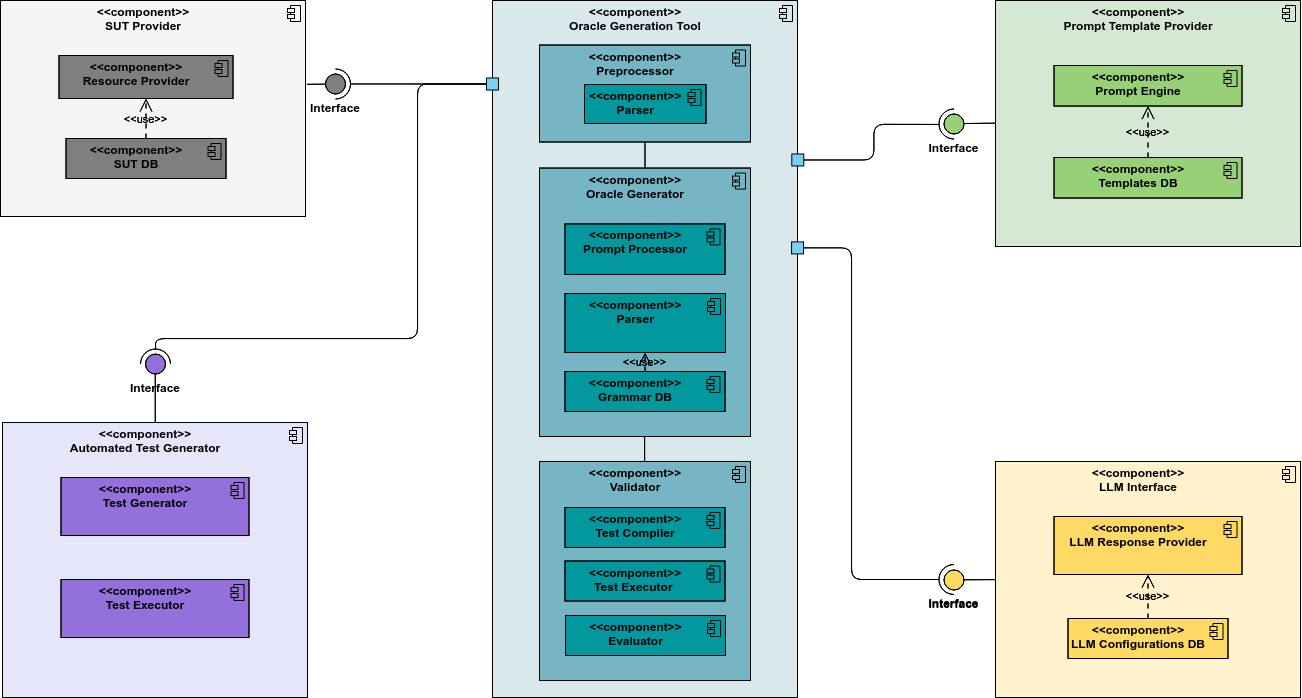
\includegraphics[width=1\textwidth]{images/EvoOracle_ components.png}
\caption{Components of our proposed approach: EvoOracle}
\label{fig:component_diagram}
\end{figure}

\vspace{0.1 cm}
\subsection{Preprocessor}
\label{subsec:preprocessor}
\vspace{0.1 cm}

    The Preprocessor is a fundamental component that analyzes the System Under Test (SUT) by parsing its code. It systematically examines each project, extracting vital details about classes and methods, along with their associated metadata. Additionally, the component identifies and establishes connections with test classes generated by the automated test generation component. It facilitates mapping each test case within a test class to the corresponding focal method. The preprocessor incorporates a parser component, which plays a pivotal role in extracting metadata linked to identified classes and methods. By traversing the project folder and locating source files, the parser parses each class file into an Abstract Syntax Tree (AST). This process collects essential information such as class names, signatures, superclasses, bodies, annotations, interfaces, package details, imports, fields, arguments list, constructors, dependencies and variables, method names, return types, and any developer-written comments. While navigating the AST, EvoOracle gathers information at both class and method levels. This parsed code serves a dual purpose: pinpointing test cases and their corresponding focal methods, and enhancing focal methods by incorporating contextual information. This component is also responsible for processing test cases generated by the Automated Test Generator. This generator produces a test suite for each target class, considering criteria like line coverage, branch coverage, configuration, and budget. With the inclusion of placeholders and focal methods, it prepares the context for LLM prompting. The Oracle Generator adopts a two-step approach, employing specific heuristics to preprocess test cases. This ensures that the test cases are adequately prepared for assertion generation, following these steps:
    \begin{enumerate}
        \item \textbf{Removal of Assertions:} All selected test cases undergo the removal of assertions, retaining only the last assertion in case there are multiple assertions using Algorithm~\ref{algorithm_remove_assertion}. This decision is based on the likelihood that reaching the last assertion implies satisfaction of all preceding assertions. This is a reasonable choice which is also seen in the work of Tufano et al. \cite{tufano_generating_2022}. The purpose is to streamline the test cases for further processing.

        \item \textbf{Placeholder Insertion:} Following the removal of additional assertions, the test cases are left with a single assertion. We replace this single assertion with a placeholder using Algorithm~\ref{algorithm_placeholder_insertion}. This placeholder serves as a temporary marker and will be subsequently replaced with assertions generated by the Large Language Models.
    \end{enumerate}

    \begin{algorithm}[H]
        \caption{Algorithm for \texttt{Removing all assertions but last}}
        \label{algorithm_remove_assertion}
        \begin{algorithmic}[1]
        \Function{remove\_all\_assertions\_but\_last}{$\text{source\_code}$}
            \State $\text{assertion\_patterns} \gets$ [\texttt{...}] \Comment{List of assertion patterns}
            \State $\text{assertions} \gets \text{FIND ALL(assertion\_pattern, source\_code)}$
        
            \If{\text{NO assertions}}
                \State \textbf{return} $\text{source\_code}$
            \EndIf
        
            \State $\text{replaced\_assertions} \gets []$
        
            \For{$i$ \textbf{in} \text{range}(\text{len(assertions) - 1})}
                \State $\text{source\_code} \gets \text{SUBSTITUTE (assertion\_pattern, "", source\_code, count=1)}$
                % \State $\text{replaced\_assertions.append(assertions[i][0] + assertions[i][1] + "();")}$  % Uncomment this line if you want to keep track of removed assertions
            \EndFor
        
            \State \textbf{return} $\text{source\_code}$
        \EndFunction
        \end{algorithmic}
        \end{algorithm}

        \begin{algorithm}[H]
        \caption{Algorithm for \texttt{Placeholder insertion}}
        \label{algorithm_placeholder_insertion}
        \begin{algorithmic}[1]
        \Function{replace\_assertions}{$\text{source\_code}$}
            \State $\text{assertion\_patterns} \gets$ [\texttt{...}] \Comment{List of assertion patterns}
            \State $\text{replaced\_assertions} \gets$ [] \Comment{List to store replaced assertions}
        
            \For{$\text{pattern}$ \textbf{in} $\text{assertion\_patterns}$}
                \Function{replacement}{$\text{match}$}
                    \State $\text{matched\_text} \gets \text{TRY MATCH}$
                    \State $\text{replaced\_assertions.append(matched\_text)}$
                    \State \textbf{return} \texttt{(ASSERTION\_PLACEHOLDER)}
                \EndFunction
        
                \State $\text{source\_code} \gets \text{SUBSTITUTE (pattern, replacement, source\_code)}$
            \EndFor
        
            \State \textbf{return} $\text{source\_code, replaced\_assertions}$
        \EndFunction
        \end{algorithmic}
        \end{algorithm}
    
\vspace{0.1 cm}
\subsection{Oracle Generator}
\label{subsec:oracle_generator}
\vspace{0.1 cm}

    The Oracle Generator is a critical component for preparing prompts and generate Oracles using LLM interface. This component is combined with several sub-components as follows:

    \begin{enumerate}
        \item \textbf{Prompt Templates:} This component utilizes prompt templates in creating a focal context tailored for each Class Under Test (CUT) and its corresponding Method Under Test (MUT). These templates serve as the foundation for replacing the contextual placeholders with the specific contexts of interest. This dynamic approach ensures that the LLMs receive targeted and meaningful prompts, enhancing their understanding of the given code context and enabling them to generate assertions with precision.

        \item \textbf{Prompt Generation Algorithm:} To create effective prompts for the Large Language Models, this component gathers information to build the context for a test case that was prepared in the preprocessing phase. This information includes key details about the class under test, methods under test, and various method attributes such as Constructor signature, Class Signature, parameters, Invoked Method Signature, dependencies, return type, developer comments, source code for the test case, package, imports, Fields, and getter/setter signature. We carefully consider all invoked methods and dependencies encapsulated within the test case. To improve the Oracles generated by the automated test generation tools, we propose the inclusion of LLMs into the test generation process. LLM Interface component provides empowers developers to tailor their LLM choices, ensuring compatibility and aligning with their project requirements and provides response. In instances where the LLM response faces challenges such as token limit exceeds, we dynamically adjust the context size. An iterative process is followed as shown in Algorithm~\ref{algorithm_prompt_generation} of generating prompts for the LLM, involving multiple rounds. Each round refines the prompt based on the LLM's response and aims to address potential challenges like token limit exceedance. The trimming process, controlled by conditional statements, adjusts the size of critical elements such as method details and test method code. By default, all the invoked method within a test case will be added to the context. Then each new attempt will reduce the method count and only keeping the details for focal method in the context. This adaptive approach ensures that the prompt remains concise while retaining essential contextual information. The code systematically handles different trimming scenarios in each round, progressively refining the prompt to strike a balance between informativeness and LLM response feasibility. The overall mechanism involves generating messages from prompt templates, seeking LLM responses, and dynamically adjusting the prompt for subsequent iterations, all of which contribute to an effective and tailored interaction with the LLM. Throughout each iteration, we analyze LLM responses to capture assertions using the specified Assertion regex. When the parsing operation successfully identifies an assertion, we advance to the subsequent phase of crafting the test case with EvoOracle assertion. In cases where the assertion parsing is unsuccessful, we continue the iteration process until we reach the budget limit specified in the configuration. 

        \begin{algorithm}
            \caption{Prompt Generation Algorithm}
            \label{algorithm_prompt_generation}
            \begin{algorithmic}[1]
                \Function{generate\_prompt}{$\text{context}$}
                    \State $\text{rounds}, \text{max\_attempts}, \text{prompt\_template} \gets []$ \Comment{No. of Iterations, attempts, prompt template}
                    \State $\text{prompts\_and\_responses} \gets []$
                    
                    \While{$\text{rounds} < \text{max\_attempts}$}
                        \State $\text{steps}, \text{rounds} \gets 0, \text{rounds} + 1$
                        \If{$\text{rounds} > 2$}
                            \State $\text{trimmed\_context} \gets \text{trim\_context(context, 3)}$ \Comment{Trim context by reducing invoked Methods details}
                        \EndIf
                        
                        \If{$\text{rounds} > 1$}
                            \State $\text{trimmed\_context} \gets \text{trim\_context(context, 5)}$ \Comment{Trim context by reducing invoked Methods details}
                        \EndIf
                        
                        \State $\text{messages} \gets \text{generate\_messages(prompt\_template, trimmed\_context)}$
                        
                        \State $\text{llm\_result} \gets \text{ask\_openLLM(messages)}$
                        \State $\text{prompts\_and\_responses.append(\{"prompt": messages, "response": llm\_result\})}$
                        
                        \State $\text{source\_code, replaced\_assertions} \gets \text{replace\_assertions(source\_code)}$
                        
                        \If{$\text{assertions}$ NOT GENERATED}
                            \State $\text{context} \gets \text{update\_prompt\_and\_ask\_again(context)}$
                        \EndIf
                    \EndWhile
                    
                    \State $\text{print\_and\_save\_results(prompts\_and\_responses)}$
                \EndFunction
            \end{algorithmic}
        \end{algorithm}
    \end{enumerate}

\vspace{0.1 cm}
\subsection{Validator}
\label{subsec:validator}
\vspace{0.1 cm}

    This component follows heuristics to evaluate the quality of the generated tests. After receiving a response from LLM interface, EvoOracle extracts and validates the assertions while selecting a different prompt modifications if any errors are detected during the validation process. 
    \begin{enumerate}
        \item \textbf{Extract:} We follow a generalized approach for extracting tests from responses. EvoOracle employs regular expressions to identify strings that matches with a set of predefined assertion formats. If EvoOracle fails to extract any assertions from LLM’s response, the whole process starts again for the next attempt with a modified prompt. Otherwise, it is considered that there is no syntactic error and the assertion is replaced back from the test case we prepared earlier.
        \item \textbf{Compile and run:} In this step, EvoOracle compiles and executes the test. If the test fails to compile or encounters errors during execution, it proceeds to the next attempt. A test is considered passed only if it is free from syntax errors, compiles successfully, runs without errors.
        \item \textbf{Mutation testing:} If a test compiles and runs without any errors, it is already an indication that the candidate tests are good enough. Another criteria is to run mutation testing on the generated tests and select only those tests which has higher mutation score.
    \end{enumerate}

At this stage, when an Oracle is successfully generated, we proceed by taking the previously prepared test case with a placeholder, as explained in Section~\ref{subsec:preprocessor}, and substitute that placeholder with the newly generated assertion. In the preprocessing stage, we had removed all the assertions except the last one. Therefore, from the response obtained from the LLM, we only consider the last assertion as well. Once the replacement is complete, we attempt to compile and run this modified test case. If
both operations are successful, we mark this test case as final. However, if any of these operations fail, we revert to the previous step of asking the LLM for another round with an updated prompt to continue refining the test case until success is achieved.

Figure~\ref{fig:evooracle_overview} shows the overview of EvoOracle's components in action.

\begin{figure}[H]
\centering
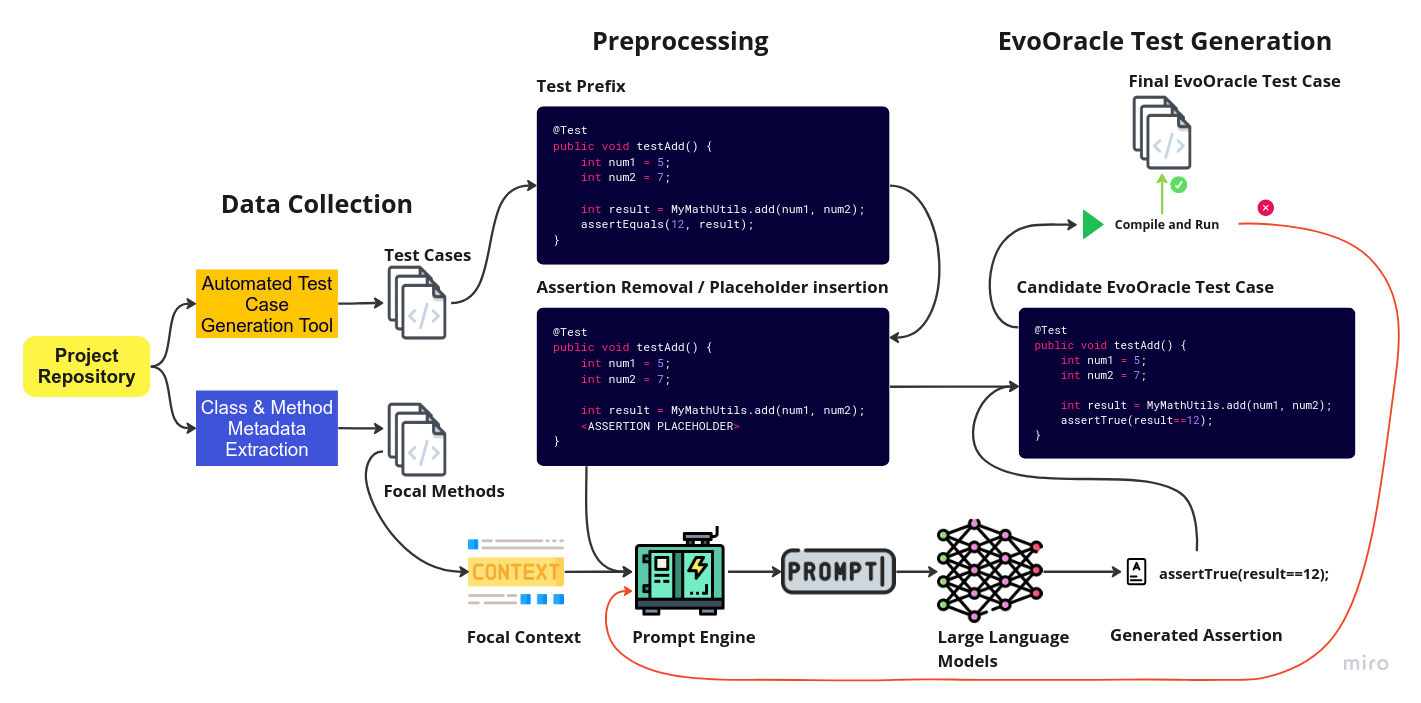
\includegraphics[width=1\linewidth]{images/evooracle_overview.png}
\caption{Overview of EvoOracle}
\label{fig:evooracle_overview}
\end{figure}

\section{Implementation}
\label{sec:implementation}
\vspace{0.2 cm}
The EvoOracle tool implements the approach presented in previous section~\ref{sec:approach} for generating Oracles for JUnit test cases in Java code. The implementation details along with all the technologies used and the choices made will be described in this section. The source code for our implementation of the tool can be found in the added references~\cite{evooracle_github}.

\vspace{0.1 cm}
\subsection{Preprocessor}
\label{subsec:preprocessor_implementation}
\vspace{0.1 cm}

\begin{enumerate}
    \item \textbf{Automated test Generator:} Our tool is designed to enhance existing test cases by focusing on improving assertions. To achieve this, we require one or more test suites, and for our implementation, we've opted to use EvoSuite. EvoSuite\cite{noauthor_evosuite_nodate} is a sophisticated tool specifically tailored for automatically generating test cases with assertions for Java code. It employs a unique hybrid approach that not only generates but also optimizes entire test suites to fulfill specific coverage criteria. These criteria guide the tool in producing comprehensive test suites that effectively cover the targeted code. EvoSuite doesn't stop at merely generating tests; it goes a step further by suggesting potential oracles for these test cases. Oracles, in this context, are sets of assertions strategically added to succinctly summarize the current behavior of the code. These assertions serve a crucial role—enabling developers to identify deviations from expected behavior and capturing the existing behavior to safeguard against potential defects in the future. We are using EvoSuite 1.0.6 release\cite{EvoSuite_release}.
    
    \item \textbf{Parsing:} In the parsing phase, we thoroughly analyze each project using the tree-sitter parser\cite{noauthor_tree-sitterintroduction_nodate}. This process involves extracting valuable metadata linked to the identified classes and methods within the project. The collected information encompasses crucial details like class names, signatures, super class, bodies, annotations, interfaces, package, imports, fields, arguments list, constructors, dependencies and variables, method names, return types, any developer written comments. This parsed code serves a dual purpose: firstly, to pinpoint test cases and their corresponding focal methods, and secondly, to enhance the focal methods by incorporating focal context information.
                                
    \item \textbf{Identify Test Classes:} In this stage, our goal is to locate all the test classes within the project. Test classes are those classes housing at least one method annotated with the \textit{\textbf{@Test}} annotation. This specific annotation serves as an indicator to JUnit, signaling that the attached method is eligible to be executed as a test case. By identifying and marking classes in this manner, we establish a clear distinction between regular classes and those instrumental to the testing process. This categorization allows a systematic approach to handling test-related components.

    \item \textbf{Identify Focal Classes:} Identifying Focal Classes involves determining the class under test for each test class. We employ a two-step approach using the following heuristics:
        \begin{enumerate}
            \item \textbf{Extracting Class Instances:} The initial heuristic involves analyzing each test method to identify all the classes instantiated or any objects created during the testing process.
            \item \textbf{Matching Class Names:} Subsequently, we employ name matching as the second heuristic. Test classes typically follow a naming convention that includes the name of the focal class, often with a \textit{"Test"} prefix or suffix. For instance, a test class associated with the \textit{"BaseSettings.java"} class might be named \textit{"BaseSettingsTest.java"} or, in the case of Evosuite, \textit{"BaseSettings\_ESTest.java."} To identify the focal class, we perform name matching by comparing the name of the test class (minus the optional \textit{"\_ESTest"} suffix) with potential focal classes. This step ensures a robust association between test classes and their corresponding focal classes.
        \end{enumerate}

    \item \textbf{Identify Focal Method:} Determining the focal method for each test case involves employing specific heuristics. 
  \begin{enumerate}
      \item \textbf{Matching Method Names:} This heuristic leverages the common practice of naming test cases similarly to their corresponding focal methods. This involves matching test case names with focal methods, considering potential prefixes or suffixes like "Test."
      \item \textbf{Analyzing Method Invocations:} Additionally, this heuristic is applied if the initial method doesn't identify a focal method. We try to match the last method invocation before (or within) the assert statement within the test case and the methods defined in the focal class. If a match is found, it is selected as the focal method. We also collect other method invocations as it might be useful to prepare the focal context. This approach is grounded in the confidence gained from prior matching of the test class to the focal class, making it likely that the test case is specifically targeting that single method.
  \end{enumerate}

  Following these heuristics, we obtain a set of test cases paired with their corresponding focal class and focal methods. Test cases where we couldn't identify the focal method using our heuristics are excluded from further consideration.

  \item \textbf{Test Case Preprocess:} We used the regex pattern shown in Listing~\ref{assertions_regex} and implemented Algorithm~\ref{algorithm_remove_assertion} and Algorithm~\ref{algorithm_placeholder_insertion} for removal of assertions and placeholder insertion. We replace the assertion with \textit{"\_\_ASSERTION\_PLACEHOLDER\_\_"} placeholder. 
      
\end{enumerate}

%Assertion selection Regex highlighting
\hrule
\begin{lstlisting}[language=Python, caption=Assertion selection Regex, label=assertions_regex]
assertion_patterns = [
    r'(\w+\.)?assert\s*\(.+?\);',           # ClassName.assert(...)
    r'(\w+\.)?assertTrue\s*\(.+?\);',       # ClassName.assertTrue(...)
    r'(\w+\.)?assertNull\s*\(.+?\);',       # ClassName.assertNull(...)
    r'(\w+\.)?fail\s*\(.+?\);',             # ClassName.fail(...)
    r'(\w+\.)?assertFalse\s*\(.+?\);',      # ClassName.assertFalse(...)
    r'(\w+\.)?assertNotEquals\s*\(.+?\);',  # ClassName.assertNotEquals(...)
    r'(\w+\.)?assertEquals\s*\(.+?\);',     # ClassName.assertEquals(...)
    r'(\w+\.)?assertArrayEquals\s*\(.+?\);',# ClassName.assertArrayEquals(...)
    r'(\w+\.)?assertNotNull\s*\(.+?\);',    # ClassName.assertNotNull(...)
    r'(\w+\.)?assertNotSame\s*\(.+?\);',    # ClassName.assertNotSame(...)
    r'(\w+\.)?assertSame\s*\(.+?\);',       # ClassName.assertSame(...)
    r'(\w+\.)?assertThat\s*\(.+?\);',       # ClassName.assertThat(...)
]
\end{lstlisting}
\hrule
    
\vspace{0.1 cm}
\subsection{Oracle Generator}
\label{sec:oracle_generator_implementation}
\vspace{0.1 cm}

\begin{enumerate}
    \item \textbf{Prompt Template:} 
    In the critical phase of prompting the Large Language Models for assertion generation, we employ a meticulous approach. To facilitate this process, we construct prompt templates using the versatile Jinja2\cite{noauthor_jinja_nodate} template format. The essence lies in creating a focal context tailored for each Class Under Test (CUT) and its corresponding Method Under Test (MUT). These templates serve as the foundation for replacing the contextual placeholders with the specific contexts of interest. This dynamic approach ensures that the LLMs receive targeted and meaningful prompts, enhancing their understanding of the given code context and enabling them to generate assertions with precision. The use of Jinja2 templates not only streamlines the prompt generation process but also allows for flexibility and adaptability in accommodating diverse code structures across different classes and methods.

    \item \textbf{LLM Integration:} To improve the Oracles generated by the automated test generation tools, we propose the inclusion of LLMs into the test generation process. Recognizing that LLMs typically demand substantial resources and powerful hardware, we opted to leverage GPT4All~\cite{noauthor_gpt4all_nodate} to make this solution accessible to developers on standard development machines. For the processing of prompts and connecting a language model to sources of context (prompt instructions, few shot examples, content to ground its response in, etc.) we use an open source framework called LangChain\cite{langchain}.

    \textbf{GPT4All:} The GPT4All~\cite{noauthor_gpt4all_nodate} project, initiated by Nomic AI, seeks to provide widespread access to Large Language Models by enabling training and deployment on common hardware. This open-source ecosystem facilitates the integration of LLMs into applications without the need for costly platform subscriptions or specialized hardware. Notably, GPT4All addresses accessibility by providing pretrained models with reduced sizes, ensuring they can operate efficiently on CPUs, even on PCs lacking internet connectivity or a GPU. This innovation allows smaller entities and independent researchers to harness LLMs for various applications, such as content creation, coding, document comprehension, and information retrieval. With a user-friendly one-click installer, GPT4All streamlines the process, making LLM utilization feasible on modern PCs with 4–16GB of RAM, a substantial reduction compared to traditional requirements, thanks to neural network quantization~\cite{han_deep_2016}.
    
    \textbf{LangChain:} LangChain\cite{langchain} stands as a versatile framework designed to empower the creation of applications driven by language models. It simplifies the process of building and training Large Language Models (LLMs) through a user-friendly interface. LangChain goes a step further by offering a selection of ready-to-use models tailored for different natural language processing tasks. Beyond modeling, it provides handy tools for tasks like data preprocessing, model evaluation, and the deployment of applications, offering a comprehensive solution for language-driven application development.
\end{enumerate}
    
\vspace{0.1 cm}
\subsection{Validator}
\label{sec:validator_implementation}
\vspace{0.1 cm}

\begin{enumerate}
    \item \textbf{Compile and Run:} 
    We use Evosuite Standalone Runtime v1.0.6\cite{noauthor_evosuite-standalone-runtime106_nodate}, JUnit v4.12\cite{noauthor_junit4.12_nodate} and Hamcrest-core v1.3\cite{noauthor_javaHamcrest_nodate} for compilation and execution of the test cases. The commands we use to compile and run are as follows:
    
\begin{verbatim}
COMPILE: javac -cp $CLASSPATH testFile
\end{verbatim}
\begin{verbatim}
RUN: java -cp $CLASSPATH org.junit.runner.JUnitCore package.testFile
\end{verbatim}

    \item \textbf{Mutation Testing Execution:} To evaluate the generated tests, we use PIT\cite{noauthor_pit_nodate} Mutation testing. PIT is a mutation testing tool that evaluates the robustness of a test suite by introducing mutations (faults) into the source code and assessing whether the tests can detect these mutations. We are using Pitest version 1.15.0\cite{noauthor_maven_nodate} by adding it to the project pom.xml file.
    
    \item \textbf{Report Parsing:} When we execute \textit{mvn pit test}, it triggers the generation of Mutation Coverage reports as artifacts. These reports provide valuable insights into the effectiveness of our test suite. To extract meaningful information, we begin by parsing the HTML reports generated by PIT. By parsing the HTML reports, we extract detailed information on line coverage, mutation coverage, and test strength for all tests associated with a particular class. This information is essential for evaluating the thoroughness and fault-detection capability of our test suite.
\end{enumerate}